\documentclass[12pt, a4paper]{book}

\usepackage[headings]{fullpage}
\usepackage{setspace}
\usepackage{graphics}
\usepackage{graphicx}
\usepackage{float}
\usepackage{subfig}
\usepackage{array}
\usepackage{multirow}
\usepackage{booktabs}
\usepackage{appendix}
\usepackage[pdfborder={0 0 0}, colorlinks=true, linkcolor=black, citecolor=blue]{hyperref}
\usepackage[printonlyused]{acronym}
\usepackage{algorithm}
\usepackage{algorithmic}
\usepackage{ifpdf}
\usepackage[utf8]{inputenc}


\graphicspath{{images}}

\newcommand{\keywords}{Brain Computer Interface, BCI, Machine Learning, ML, P-300, P-300 Speller, On-Screen Keyboard, Keyboard}
\newcommand{\submissionDay}{26}
\newcommand{\submissionMonth}{May}
\newcommand{\submissionYear}{2019}
\newcommand{\submissionDate}{\submissionDay~\submissionMonth,~\submissionYear}
\newcommand{\typeOfThesis}{Bachelor Thesis - Expository}
\newcommand{\titleOfThesisOne}{A Brain-controlled On-screen Assistive Keyboard}
\newcommand{\authorOfThesis}{Maqarios Wagdy Tawadros Saleh Mohareb}
\newcommand{\supervisor}{Assoc. Prof. Seif Eldawlatly}

\newcommand{\figureWidth}{100mm}
\newcommand{\subFigureWidth}{70mm}

\ifpdf
\pdfinfo {
	/Author (\authorOfThesis)
	/Title (\titleOfThesisOne)
	/Subject (\typeOfThesis)
	/Keywords (\keywords)
}
\fi




\begin{document}


\pagestyle{plain}

\newcommand{\titlePage}{
    \thispagestyle{empty}
    \begin{center}
    	\textbf{Media Engineering and Technology Faculty}\\[1mm]
    	\textbf{German University in Cairo}\\[1mm]
    	
\includegraphics[width=3cm]{images/title_page/GUC_logo.jpg}
    	
    	\vspace{2cm}
    	\doublespacing
    	{\Huge \textbf{\titleOfThesisOne}}\\
    	\singlespacing
    	\vspace{2cm}
    	{\large \textbf{\typeOfThesis}}\\
    	
    	\vfill
    	\parbox{1cm}{
      		\begin{large}
        			\begin{tabbing}
           			Author: \hspace{2cm}  
            			\=\authorOfThesis\\[2mm]
          			Supervisors: 
            			\>\supervisor\\[2mm]
          			Submission Date: 
            			\>\submissionDate\\
        			\end{tabbing}
      		\end{large}
    	}\\
    \end{center}
    \clearpage
}


\titlePage
\thispagestyle{empty}\ \clearpage
\titlePage


\thispagestyle{empty}
This is to certify that:
\begin{itemize}
\item[(i)] the thesis comprises only my original work toward the Bachelor Degree
\item[(ii)] due acknowledgement has been made in the text to all other material used
\end{itemize}

\vspace{2cm}
\begin{flushright}
\rule[0mm]{6cm}{0.2mm}\\
\authorOfThesis\\
\submissionDay~\submissionMonth,~\submissionYear\\
\end{flushright}
\clearpage
\chapter*{Acknowledgments}\label{chap:acknowledgments}

\paragraph{}
First of all, I would like to express my at-most gratitude to my supervisor Assoc. Prof. Seif El-Dawlatly for his support and immense knowledge. His sincere guidance helped me a lot in the time of research, application, experimentation and writing of this thesis.

\paragraph{}
Besides my supervisor, I thank my colleagues Ahmed Alaa, Mostafa Nasr and Omar Ashraf for giving me insightful arguments and collection of data.

\paragraph{}
Last but not least, I would like to thank my parents for the continuous support and patience.
\chapter*{Abstract}
\label{chap:abstract}
% ================================================================
In this project, an on-screen keyboard will be made. The main aim of this project is to help people with physical disability use computers more easily.\par
% ----------------------------------------------------------------
Using \ac{p300} based \ac{bci} which uses oddball paradigm to determine the required actions to be done by the application. By displaying a matrix of characters, the user can determine the character he wants from this matrix.\par
% ----------------------------------------------------------------
By processing the recorded brain waves to \ac{ml} model and apply mathematical filters to accurately determine the intended actions. Thus, reaching an accuracy with an average of 80\% in character recognition rate which is not bad compared to previous results obtained by previous papers \cite{inproceedings1, inproceedings2, article1, article2}.\par
% ----------------------------------------------------------------
\clearpage
% ================================================================

\tableofcontents
\clearpage 
\pagestyle{headings}
\setlength\parskip{.5\baselineskip plus .2\baselineskip
	minus .4\baselineskip}

\subsubsection{Motivation}
Imagine that one day, while you are setting on the bed too lazy to move. with this project all you need to do, is just one glance at the computer screen near you to send an email to your employer telling him that you are not coming today. Or having a disabled friend but wants to learn programming. all of these are possible using brain waves, In a parallel world brain waves is a synonyms for laziness.
\subsubsection{Objective}
The aim of this project is to build on-screen keyboard however without using clicks but brain waves to choose a character within a matrix.
\subsubsection{Brief Description}
A matrix of characters (i.e. 6x6) each cell has a character. The matrix is displayed for a certain period then each row and column will be intensified for a certain period of time randomly. The row and column which has a certain wave form is their intersection is the chosen character.
\section{Introductory to BCIs}
BCI Stands for (Brain-Computer Interface) which refers to intercepting the brain waves through some means such as electrodes, which is then transmitted to a computer after amplifying and digitizing the signal (Figure 2.1). The process starts with the intent of the user to do some action such as raising the right hand, the BCI records the brain activity and sends the intercepted signals to the BCI applications to do the desired reaction. There are several terms such as BMI (Brain-Machine Interface) or DBI (Direct Brain Interface) have the same meaning as BCI, however there are some terms such as Neuroprosthesis are not the same because BCI refers to only receiving (intercepting) data from the brain, however Neuroprosthesis refers to both sending and receiving data to and from the brain. In other words, BCI is a subset of Neuroprosthesis.
\begin{figure}
    \centering
    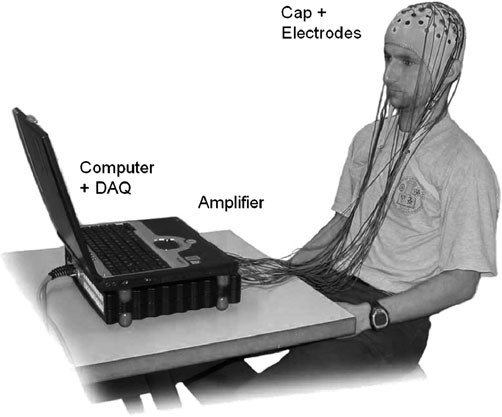
\includegraphics[width=70mm]{images/figure-2-1.jpg}
    \caption{Person records BCI data}
    \label{fig:my_label}
\end{figure}


\subsection{Processes of Operation}
BCI goes through three main procedures, measuring the brain activity, processing it and controlling the intercepted signals.
\subsubsection{Measuring Brain Activity}
Brain activity produces magnetic and electrical waves. That’s why, sensors or electrodes are used to measure these changes at different areas and times. Brain activities can be recorded through sensors (non-surgical solution) or electrodes (surgical solutions). For the non-surgical solution, sensors are used to measure the electrical activity from the scalp and this solution is called Electroencephalography (EEG) (Figure 2.1). They are relatively easy to deal with however they don’t provide accurate measures due to external interference and are susceptible to limitations in frequency range. In order to get consistent recording, sensors are spread on the scalp through system called 10 - 20 (Figure 2.2). 10 - 20 refers to how sensors are spread 10 - 20 - 20 - 20 - 20 - 10 percent. The 6 regions are named according to their position: Fp - pre-frontal, F - frontal, C - central, P - parietal, O - occipital, T - temporal. On the other hand, the surgical solution need to open the skull through surgical procedures and plant the electrodes. When the electrodes are planted on the surface of the cortex, it’s called electrocorticogram (ECoG). And another solution called Intracortical, which plants the electrodes in the inner parts of the brain. Although the surgical solutions provide higher accuracy and frequency range compared to the non-surgical solution they have serious drawbacks such as they need surgery, finance and can have ethical problems. Difference between each solution is shown in Figure 2.3.
\begin{figure}
    \centering
    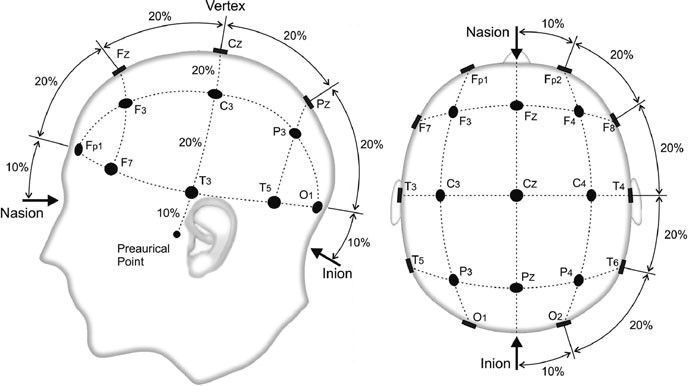
\includegraphics[width=70mm]{images/figure-2-2.jpg}
    \caption{10 - 20 System that shows how sensors are spread on the scalp}
    \label{fig:my_label}
\end{figure}
\begin{figure}
    \centering
    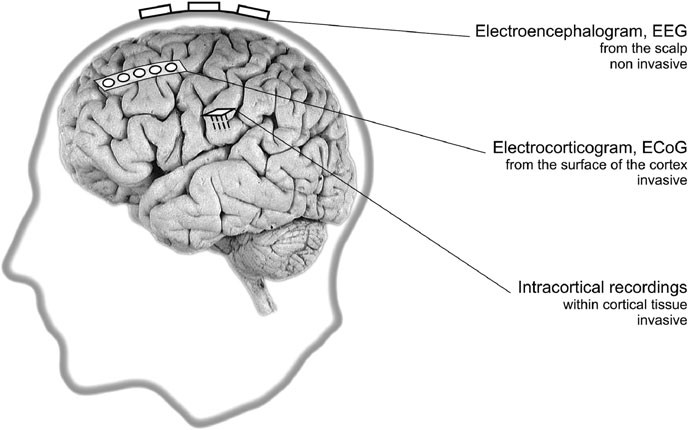
\includegraphics[width=70mm]{images/figure-2-3.jpg}
    \caption{Types of Reading Brain Waves on Computers (BCIs)}
    \label{fig:my_label}
\end{figure}

\subsubsection{Process and Control}
Processing and Controlling Received Signals are handled within the application.

\subsection{Brain Patterns}
Because measuring brain activity is not enough, some mental strategies are used to trigger the required tasks. The most used mental strategies are selective attention and motor imagery.
\subsubsection{Selective Attention}
Mental strategies based on selective attention require external stimuli such as auditory stimuli or visual stimuli. P300 (Peak signal at 300ms) or SSVEP (Steady-State Visual Evoked Potentials) are two mental strategies the depends on visual stimulation. P300 is triggered when the intensity of symbols is changed and SSVEP is triggered with flickering some areas with certain frequencies (6 – 30Hz).


\section{Online Dataset}
BCI2000, Competition III, Dataset II.

\subsection{Paradigm}
The user was shown a 6 by 6 matrix containing English letters and numbers (Figure 2.4). The user was to spell words and focus his attention of the character that he wants to choose. All rows and columns were intensified randomly and successively at a rate of 5.7Hz (100ms intensification, 75ms no intensification). In other words, a column or row is intensified (i.e. row 2 in Figure 2.4) for 100ms then, no row or column is intensified for 75ms, then repeat. The row and column (2 intensifications) which contained the chosen character will provide different signals (P300) compared to the other 10 intensifications which does not contain the chosen character (Non-P300).
\begin{figure}
    \centering
    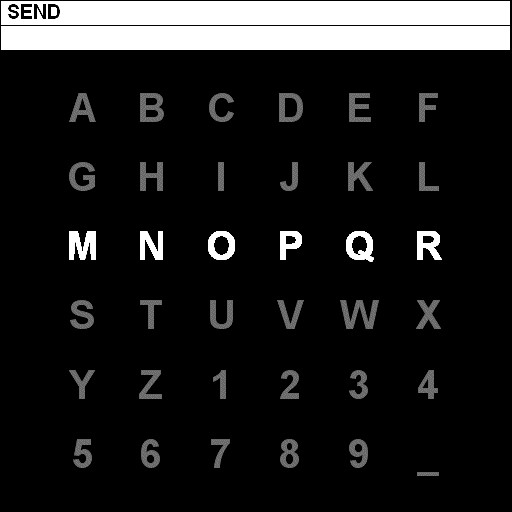
\includegraphics[width=70mm]{images/figure-2-4.jpg}
    \caption{The matrix displayed to the user}
    \label{fig:my_label}
\end{figure}

\subsection{Collection of Dataset}
Signals are filtered from 0.1 – 60Hz and digitized at 240Hz (Each 240 samples corresponds to 1 second). The 12 sets of intensifications were repeated 15 times for each character resulting in 180 total intensifications per epoch (character) into 64 channels EEG (Figure 2.5).
\begin{figure}
    \centering
    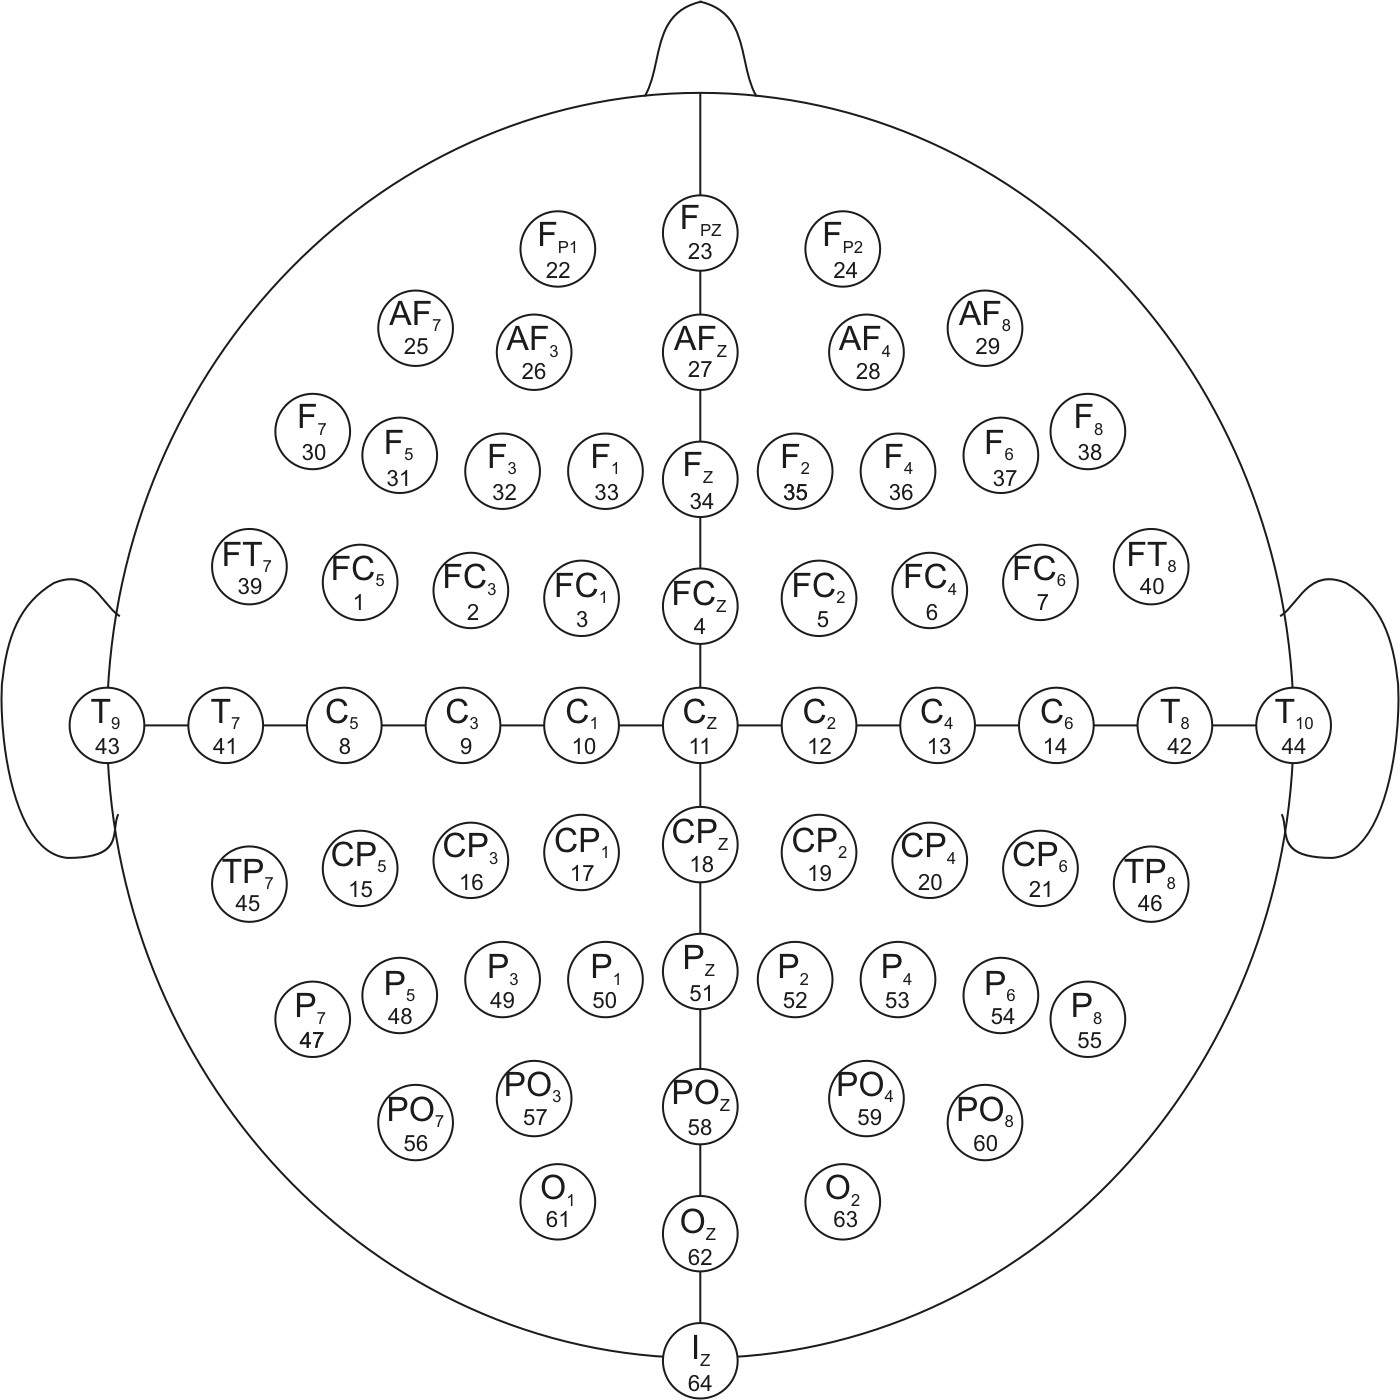
\includegraphics[width=70mm]{images/figure-2-5.jpg}
    \caption{Mapping of each sensors to its place on the scalp}
    \label{fig:my_label}
\end{figure}

\subsection{Explanation of The Dataset}
The dataset has 2 subjects (A and B), where each subject has 85 characters (epochs) in training dataset and 100 characters in testing dataset (Remember that, each epoch has 12 intensifications and 15 repetitions). The structure of variables for each subject file is described below.\newline
\begin{tabbing}
Title:\quad \quad \quad \quad \quad \=Description\kill
Signal:         \>signal of each channel (Figure 2.5)\\
                \>Type: 3D Array\\
                \>Shape (Dimension): (85, 7794, 64)\\
\newline\\
TargetChar:     \>The chosen character for each epoch\\
                \>Type: String\\
                \>Length: 85\\
\newline\\
Flashing:	    \>0	when NO row/column is intensified\\
                \>1	when row/column is intensified\\
                \>Type: 2D Array\\
                \>Shape (Dimension): (85, 7794)\\
\newline\\
StimulusCode:	\>0	when NO row/column is intensified\\
                \>1 ... 6	when intensified column (1 is left-most column)\\
                \>7 ... 12	when intensified row (1 is upper-most row)\\
                \>Type: 2D Array\\
                \>Shape (Dimension): (85, 7794)\\
\newline\\
StimulusType:	\>0	when NO row/column is intensified\\
		        \>1	when row/column contains the chosen character\\
                \>Type: 2D Array\\
                \>Shape (Dimension): (85, 7794)\\
\end{tabbing}
Note: 7794 samples because the data is digitized and there is a no-intensification period between each intensification.
Note: TargetChar, StimulusType are only provided for training dataset.

\subsection{Analysis}
Figure 2.6 shows signal wave forms for P300.
\begin{figure}
    \centering
    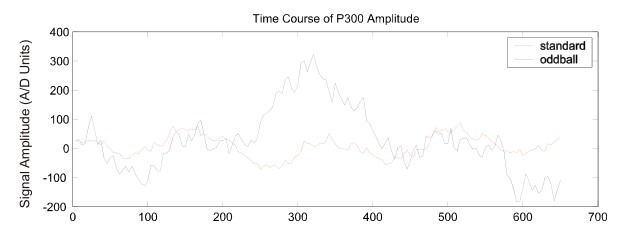
\includegraphics[width=70mm]{images/figure-2-6.jpg}
    \caption{Caption}
    \label{fig:my_label}
\end{figure}


\chapter{Approach}
\label{chap:approach}
% ================================================================
% DATA DESCRIPTION
\section{Data Description}
In this project, BCI2000, Competition III, Dataset II was used, due to being accurate, free, provides 64 channels and quite a number of papers was based on it which provides a good reference for comparison of classifiers and the corresponding accuracy. In addition to the competition's dataset, we recorded our own dataset from 2 subjects. In total, the competition's dataset has 2 subjects A and B, the recorded dataset has another 2 subjects C and D.\par
% ----------------------------------------------------------------
\subsection{Paradigm}
The \ac{p300} speller in the competition was like the following; the user is shown a 6x6 matrix of characters (Figure \ref{fig:p300-speller}). Each row and column is intensified in a random sequence. Then, the user focuses his gaze on one of the 36 cells of the matrix. The sequence of 12 intensifications (6 rows + 6 columns) which results in an oddball paradigm where the intensification of the focused character represents the infrequent event and the other intensifications + no intensifications represents the frequent event. The event which is infrequent will result in a \ac{p300} response, while the frequent event will have no change on the signal (Figure \ref{fig:p300-signal}). \cite{article1}\par
\begin{figure}
    \centering
    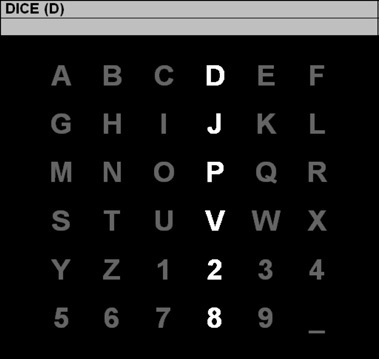
\includegraphics[width=\figureWidth]{images/approach/p300_speller.jpg}
    \caption{\ac{p300} Speller: Representation of the intensification of the 4th column \cite{article1}.}
    \label{fig:p300-speller}
\end{figure}
% ----------------------------------------------------------------
\subsection{Recording}
\subsubsection{Competition's Data}
In the competition's dataset (Subjects A and B), signals are filtered from 0.1 – 60Hz and digitized at 240Hz (Each 240 samples corresponds to 1 second). The 12 sets of intensifications were repeated 15 times for each character resulting in 180 total intensifications per epoch (character) into 64 channels EEG (Figure \ref{fig:competition-64-channels}). There are 185 epoch in total; 85 train and 100 test per subject.\par
\begin{figure}[!ht]
    \centering
    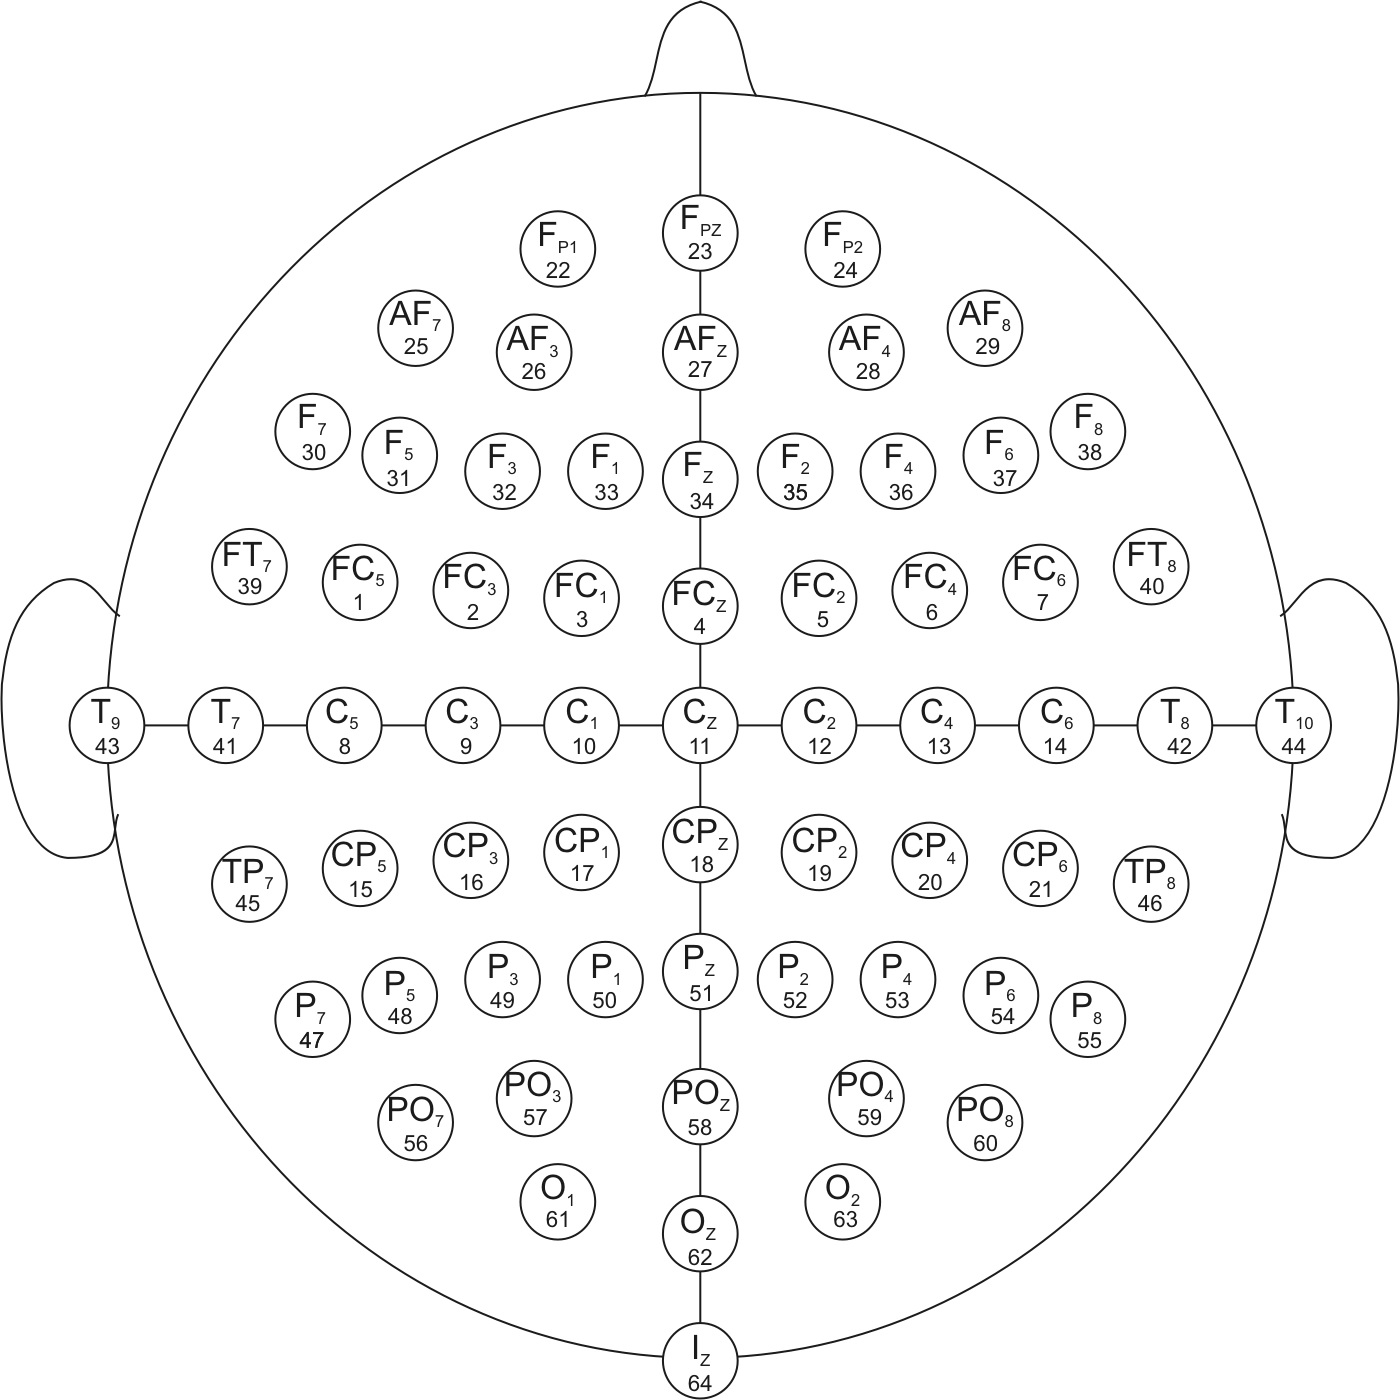
\includegraphics[width=\figureWidth]{images/approach/competition_64_channels.jpg}
    \caption{Mapping of sesnors on the scalp according to the competition's dataset description.}
    \label{fig:competition-64-channels}
\end{figure}
% ----------------------------------------------------------------
\subsubsection{Recorded Data}
In the dataset we recorded (Subjects C and D), signals are digitized at 128Hz (Each 128 samples corresponds to 1 second). The 12 sets of intensifications were repeated 15 times for each character resulting in 180 total intensifications per epoch into 14 channels EEG (Figure \ref{fig:emotiv-14-channels}, (a)). There are 72 epoch in total; 57 train and 15 test per subject.\par.
\begin{figure}
    \centering
    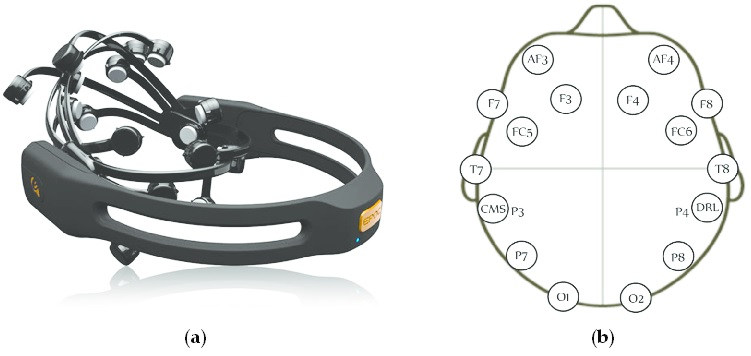
\includegraphics[width=\figureWidth]{images/approach/emotiv_14_channels.jpg}
    \caption{Mapping of sesnors on the scalp in EMOTIV EPOC+ headset \cite{article8}.}
    \label{fig:emotiv-14-channels}
\end{figure}
% ----------------------------------------------------------------
Note that, only 14 channels were recorded for subjects (C, D) due to hardware limitation (EMOTIV EPOC+). The 14 channels are AF3, F7, F3, P3, T7, P7, O1, O2, P8, T8, P4, F4, F8 and AF4 (Figure \ref{fig:emotiv-14-channels}, (b))\par
% ----------------------------------------------------------------
\subsection{Data Explanation}
\label{subsection:data-explanation}
The competition's dataset has 5 arrays descried below (the description provided by the competition for dataset 2).
\begin{tabbing}
    Title:\quad \quad \quad \quad \quad \=Description\kill
    Signal:         \>signal of each channel (Figure 2.5)\\
                    \>Type: 3D Array\\
                    \>Shape (Dimension): (85, 7794, 64)\\
    \newline\\
    TargetChar:     \>The chosen character for each epoch\\
                    \>Type: String\\
                    \>Length: 85\\
    \newline\\
    Flashing:	    \>0	when NO row/column is intensified\\
                    \>1	when row/column is intensified\\
                    \>Type: 2D Array\\
                    \>Shape (Dimension): (85, 7794)\\
    \newline\\
    StimulusCode:	\>0	when NO row/column is intensified\\
                    \>1 ... 6	when intensified column (1 is left-most column)\\
                    \>7 ... 12	when intensified row (1 is upper-most row)\\
                    \>Type: 2D Array\\
                    \>Shape (Dimension): (85, 7794)\\
                    \>Figure \ref{fig:row-column-numbering}\\
    \newline\\
    StimulusType:	\>0	when NO row/column is intensified\\
    		        \>1	when row/column contains the chosen character\\
                    \>Type: 2D Array\\
                    \>Shape (Dimension): (85, 7794)\\
\end{tabbing}\par
\begin{figure}
    \centering
    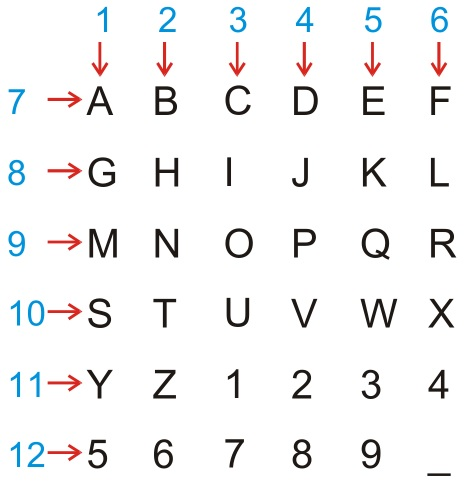
\includegraphics[width=\figureWidth]{images/approach/row_column_numbering.jpg}
    \caption{Row/Column numbering values.}
    \label{fig:row-column-numbering}
\end{figure}
% ----------------------------------------------------------------
Note: This is dimension of the train dataset. If dimension of the test dataset is needed, substitute 85 with 100.\par
% ----------------------------------------------------------------
Note: TargetChar, StimulusType are only provided for training dataset.\par
% ----------------------------------------------------------------
Note: Since algorithm has been updated, only Signal, TargetChar, StimulusCode and the matrix used for training are needed to train the \ac{ml} model.\par
% ----------------------------------------------------------------
\clearpage
% ================================================================






% DATA PRE-PROCESSING
\section{Data Pre-processing}
% ----------------------------------------------------------------
\subsection{Average of Repetitions}
Average of the all repetitions for both the competition's dataset and the recorded dataset were done according to the proposed algorithm provided by the competition in the example file. A modified version is that, we search for 2 consecutive samples in StimulusCode current and previous. If the current sample is zero, and the previous sample is non-zero, then that means there was a transition from intensification to no intensification. Then we sum the samples of the window needed (i.e. 192 samples = 800ms for competition's dataset) to the corresponding previous intensification samples.\par
% ----------------------------------------------------------------
For example, in the competition's dataset, according to Sub-Section \ref{subsection:data-explanation}, the train set has dimension (85, 7794, 64), after calculating the average the repetitions the new dimensions will be (85, 12, 192, 64).\par
% ----------------------------------------------------------------
Note: 7794 and 192 because the digitization rate for the the used headset in the competition is 240 Hz.\par
% ----------------------------------------------------------------
In the recorded dataset, the train set has dimension (57, 4600, 14), after calculating the average the repetitions the new dimensions will be (57, 12, 102, 14).\par
% ----------------------------------------------------------------
Note: 4600 and 102 because the digitization rate for the EMOTIV headset is 128 Hz.\par
% ----------------------------------------------------------------
\subsection{Filters}
\subsubsection{Common Average Reference (CAR)}
The signals were filtered using \ac{car} filter (Equation \ref{eq:car}). By subtracting the mean of samples across all channels at certain time from signals at the same certain time helps to remove the noise in some channels.\par
\begin{equation}
    f_c(t) = s_c(t) - \frac{1}{N} \sum_{i=1}^N s_i(t)
    \label{eq:car}
\end{equation}
% ----------------------------------------------------------------
$f_c(t)$ is the filtered signal for electrode (channel) c at time t. $s_c(t)$ is the raw signal for electrode (channel) c at time t. $\frac{1}{N} \sum_{i=1}^{N} s_i(t)$ is the mean of channels at time t.\par
% ----------------------------------------------------------------
\subsubsection{Moving Average}
After that, Moving average filter was applied in order to remove noise within time units per channel (Equation \ref{eq:ma}).\par
\begin{equation}
    f_c(t) =  \frac{1}{M} \sum_{i=t}^{t+M} s_c(i)
    \label{eq:ma}
\end{equation}
% ----------------------------------------------------------------
$f_c(t)$ is the filtered signal for electrode (channel) c at time t. $\frac{1}{M} \sum_{i=t}^{t+M} s_c(i)$ is the mean consecutive M signal where M is the moving average filter value.\par
% ----------------------------------------------------------------
In the competition's dataset, it will be set to 25 \cite{inproceedings1}. However, in the recorded dataset, it will be set to 13 \cite{inproceedings2}.\par
% ----------------------------------------------------------------
\subsubsection{Z-Score}
After applying moving average, the signals were scaled using Z-Score (Equation \ref{eq:zs}).\par
\begin{equation}
    f_{cj} =  \frac{s_c(j) - \mu_c}{\sigma_c}
    \label{eq:zs}
\end{equation}
% ----------------------------------------------------------------
$f_{cj}$ is the filtered signal for electrode (channel) c and feature j. $s_c(j)$ is the signals for electrode c and feature j. $\mu_c$ is the mean of signals recorded on electrode c. $\sigma_c$ is the standard deviation of signals recorded on electrode c.\par
% ----------------------------------------------------------------
\subsubsection{Decimation}
Finally, the filtered signal is decimated by certain value. Assume decimation value of n. This means we will take 1 signal as a feature every n signals.\par
% ----------------------------------------------------------------
In the competition's dataset, it will be set to 12 \cite{inproceedings1}. However, in the recorded dataset, it will be set to 6 \cite{inproceedings2}.\par
% ----------------------------------------------------------------
\clearpage
% ================================================================





% FEATURE EXTRACTION
\section{Feature Extraction}
\subsection{Channel Selection}
\label{subsection:channel-selection}
Data segments of extracted data can vary a lot since the elicited signal appears from 250 - 500ms. Most papers \cite{inproceedings1, inproceedings2, article1, article2} uses data segments that vary from 600 - 1000ms. However, in this project, 0 - 800ms data segment is going to be used.\par
% ----------------------------------------------------------------
In the competition's dataset, the number of samples will be 192 sample. There are 2 sets of channels are going to be used; the first will consist of 8 channels (Fz, Cz, Pz, P3, P4, PO7, PO8 and
Oz) (Figure \ref{fig:competition-8-channels}) \cite{inproceedings1, article1}. And the other set will consist of all the 64 channels.\par
\begin{figure}
    \centering
    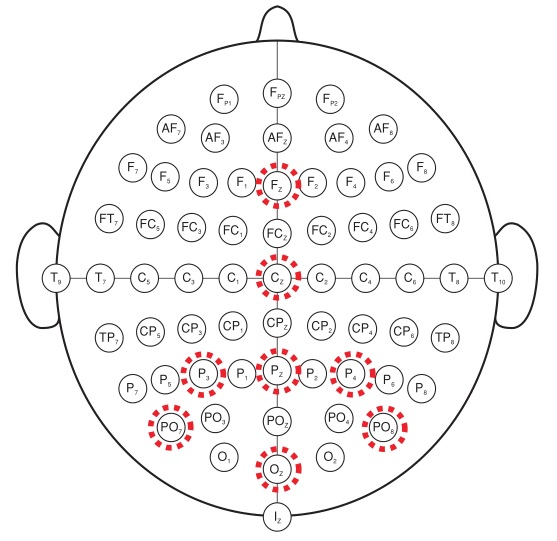
\includegraphics[width=\figureWidth]{images/approach/competition_8_channels.jpg}
    \caption{Most effective electrodes according to Dean and Sellers \cite{article1}.}
    \label{fig:competition-8-channels}
\end{figure}
% ----------------------------------------------------------------
On the other hand, then number of sample for the recorded dataset will be 102 sample. And all the 14 channels are going to be used (Figure \ref{fig:emotiv-14-channels}).
% ----------------------------------------------------------------
\subsection{Feature Vector Concatenation}
After channel selection, all the extracted channels will then be concatenated and passed to the classifier. This approach was used to allow the use of more than 1 channel to determine the \ac{p300}.\par
% ----------------------------------------------------------------
\clearpage
% ================================================================



% CLASSIFICATION
\section{Classification}
Since \ac{p300} is an oddball paradigm, meaning that it is either frequent or infrequent event. The whole classification problem is a binary one. It is either \ac{p300} or Non-\ac{p300}. In this project, linear classifiers whose decision boundary will be like Equation \ref{eq:linear-classifier-boundary}.\par
\begin{equation}
    w^T x + b = 0
    \label{eq:linear-classifier-boundary}
\end{equation}
% ----------------------------------------------------------------
$w$ is the weight (line slope). $x$ is the feature vector (sample). $b$ is the bias term (line shift).\par
% ----------------------------------------------------------------
\subsection{Class Construction and Character Prediction}
Since the problem is a binary classification problem, we will set the the target class to be 1 for the intensification with \ac{p300}, and -1 (or 0) for the intensification with Non-\ac{p300}.\par
Since the \ac{p300} Speller is only has 2 \ac{p300} events (1 for each dimension row/column), the character prediction will be based on the maximum value from the score function (decision function).\par
% ----------------------------------------------------------------
Note that, the higher the score (score is the predicted y label) (Equation \ref{eq:score}), the further away from the corresponding line on the hyper plane, which makes it more accurate for a \ac{p300} elicit (Equation \ref{eq:predicted-row}, and Equation \ref{eq:predicted-column}) \cite{inproceedings1, inproceedings2, article1}.\par
\begin{equation}
    score = w^T x
    \label{eq:score}
\end{equation}
\begin{equation}
    row = max(w^T x_{7..12})
    \label{eq:predicted-row}
\end{equation}
\begin{equation}
    column = max(w^T x_{1..6})
    \label{eq:predicted-column}
\end{equation}
% ----------------------------------------------------------------
$w$ is the weight. $x$ is the feature vector. $max(..)$ is a function to get max of given values. Check Sub-Section \ref{subsection:data-explanation} for row/column numbering values.\par
% ----------------------------------------------------------------
\subsection{Linear Discriminant Analysis (LDA)}
\ac{lda} is the most basic linear classifier which is based on least squared error. The weight vector is calculated based on Equation \ref{eq:lda-weight-calculation} \cite{inproceedings1}.\par
\begin{equation}
    w = (X^T X)^{-1} X^T y
    \label{eq:lda-weight-calculation}
\end{equation}
% ----------------------------------------------------------------
$w$ is the weight. $X$ is the matrix with feature vectors as rows. $y$ is the vector that has the labels of each row within $X$.\par
% ----------------------------------------------------------------
For Example, in the competition's dataset, $X$ has dimension (1020, 128), and $y$ has dimension (1020). Note that, we are using 85 character (train dataset), 12 intensifications, 192 sample (0 - 800ms) and 8 concatenated channel.\par
\[85 \times 12 = 1020\]
\[\frac{192}{12} \times 8 = 128\]
% ================================================================


% Graphical User Interface (GUI)
\section{Graphical User Interface (GUI)}
The language used to make the \ac{gui} is python programming language. As for the \ac{gui} package itself (classes and functions) is called Tkinter.\par
% ----------------------------------------------------------------
The user is shown the matrix in Figure \ref{subfig:recorded-gui-non-intensification} for 2.5 seconds. Then, the intensifications of rows and columns starts (12 intensifications, 15 repetitions) as in Figure \ref{subfig:recorded-gui-intensification}, after that, the \ac{gui} halts for 2 seconds because the \ac{p300} takes time to take effect (300ms after the stimulus).\par
% ----------------------------------------------------------------
Note that, number 5 is highlighted in Figure \ref{subfig:recorded-gui-non-intensification} to signify that the user should focus on it in order to train it.\par
\begin{figure}[!ht]
    \centering
    \subfloat[
        Non-intensification state of the \ac{gui} (frequent event).
        \label{subfig:recorded-gui-non-intensification}
        ]{
            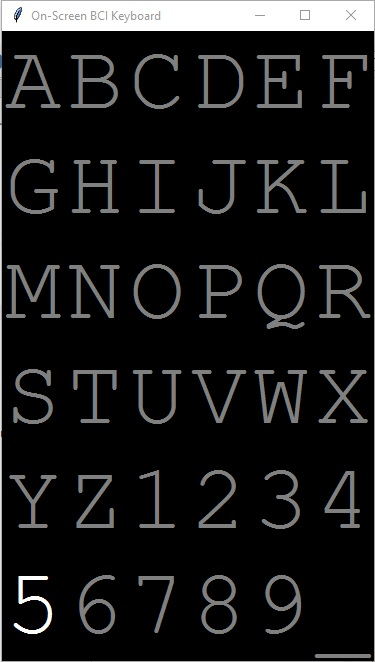
\includegraphics[width=\subFigureWidth]{images/approach/recorded_gui_non_intensification.jpg}
        }
    \hfill
    \subfloat[
        Intensification state of column 4 state of the \ac{gui} (infrequent event).
        \label{subfig:recorded-gui-intensification}
        ]{
            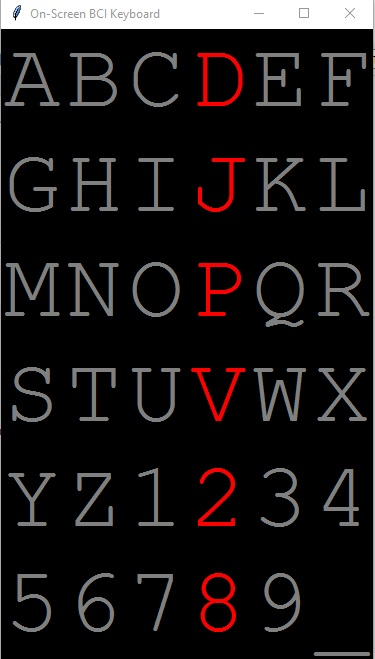
\includegraphics[width=\subFigureWidth]{images/approach/recorded_gui_intensification.jpg}
        }
    \caption{\ac{gui} used to record the dataset.}
    \label{fig:recorded-gui}
\end{figure}
% ----------------------------------------------------------------
\clearpage
% ================================================================

\chapter{Results}
\label{chap:results}
% ================================================================
\section{Competition's Dataset}
\label{section:competitions-dataset}
The user was shown a 6x6 matrix containing A..Z, 1..9 and \_ as shown in Chapter \ref{chap:approach}, Figure \ref{fig:p300-speller}. Each row and column was intensified once in a random sequence resulting in 12 intensifications in total. Each trial (12 intensification) was repeated 15 times which results in 180 total intensification per epoch. Each intensification lasts for 100ms followed by 75ms without any intensifications and so on. The above information are according to the description provided by competition 3 dataset 2.\par
% ----------------------------------------------------------------
Each subject (A and B) has 85 epoch (character) as train dataset and 100 epoch as test dataset. Figure \ref{fig:subject-A-p300} and Figure \ref{fig:subject-B-p300} shows the average of \ac{p300} plot for the 2 intensifications (row and column) that has the chosen character versus the 10 intensifications that does not contain the character.\par
\begin{figure}
    \centering
    \subfloat[
        Subject A \ac{p300} plot on train dataset on channel Cz.
        \label{subfig:subject-A-p300-train}
        ]{
            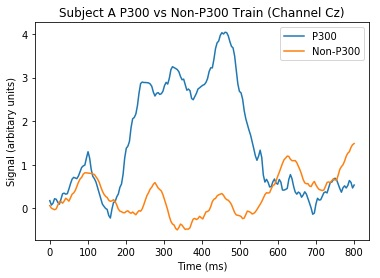
\includegraphics[width=\subFigureWidth]{images/results/subject_A_p300_train.jpg}
        }
    \hfill
    \subfloat[
        Subject A \ac{p300} plot on test dataset on channel Cz.
        \label{subfig:subject-A-p300-test}
        ]{
            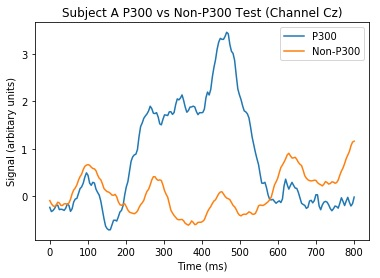
\includegraphics[width=\subFigureWidth]{images/results/subject_A_p300_test.jpg}
        }
    \caption{\ac{p300} plot of subject A.}
    \label{fig:subject-A-p300}
\end{figure}
\begin{figure}
    \centering
    \subfloat[
        Subject B \ac{p300} plot on train dataset on channel Cz.
        \label{subfig:subject-B-p300-train}
        ]{
            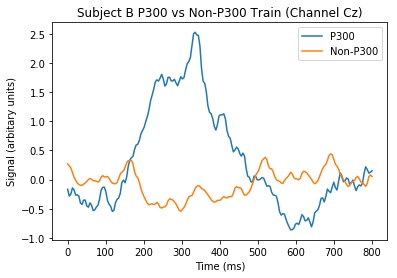
\includegraphics[width=\subFigureWidth]{images/results/subject_B_p300_train.jpg}
        }
    \hfill
    \subfloat[
        Subject B \ac{p300} plot on test dataset on channel Cz.
        \label{subfig:subject-B-p300-test}
        ]{
            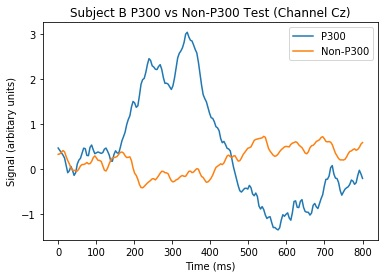
\includegraphics[width=\subFigureWidth]{images/results/subject_B_p300_test.jpg}
        }
    \caption{\ac{p300} plot of subject B.}
    \label{fig:subject-B-p300}
\end{figure}
% ----------------------------------------------------------------
Table \ref{tab:subject-A-B-char-reco} shows the character recognition analysis for subjects A and B according to the proposed channels mentioned in Sub-Section \ref{subsection:channel-selection}.\par
\begin{table}
    \centering
    \begin{tabular}{ c | c | c | c | c | c || c}
        \hline
        \textbf{Classifier} & \textbf{Channels} & \textbf{Window} & \textbf{Filters} & \textbf{A} & \textbf{B} & \textbf{Average} \\
        \hline\hline
        \multirow{8}{*}{\textbf{LDA}} & 8 & $0 \to 800ms$ & - & $73$ & $81$ & $77\pm4$\%\\
        {} & 8 & $0 \to 800ms$ & CarMaZsD & $79$ & $90$ & $84.5\pm5.5$\%\\
        
        {} & 8 & $200 \to 600ms$ & - & $71$ & $85$ & $78\pm7$\%\\
        {} & 8 & $200 \to 600ms$ & CarMaZsD & $65$ & $78$ & $71.5\pm6.5$\%\\
        
        {} & 64 & $0 \to 800ms$ & - & $81$ & $85$ & $83\pm2$\%\\
        {} & 64 & $0 \to 800ms$ & CarMaZsD & $89$ & $84$ & $86.5\pm2.5$\%\\
        
        {} & 64 & $200 \to 600ms$ & - & $86$ & $82$ & $84\pm2$\%\\
        {} & 64 & $200 \to 600ms$ & CarMaZsD & $82$ & $78$ & $80\pm2$\%\\
        \hline
    \end{tabular}
    \caption{Subject A and B character recognition rate.}
    \label{tab:subject-A-B-char-reco}
\end{table}
% ----------------------------------------------------------------
\clearpage
% ================================================================


\section{Recorded Dataset}
The same paradigm was applied as in Section \ref{section:competitions-dataset} same matrix, 12 intensifications, 15 repetitions, 100 ms for intensification and 75ms no intensification.\par
% ----------------------------------------------------------------
However, Each Subject (C and D) has 57 epoch as train dataset and 15 epoch as test dataset. Figure \ref{fig:subject-C-p300} and Figure \ref{fig:subject-D-p300} shows the average of \ac{p300} plot all 72 epochs.\par
\begin{figure}[!ht]
    \centering
    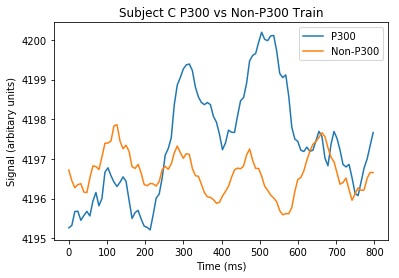
\includegraphics[width=\figureWidth]{images/results/subject_C_p300.jpg}
    \caption{Subject C \ac{p300} plot.}
    \label{fig:subject-C-p300}
\end{figure}
\begin{figure}[!ht]
    \centering
    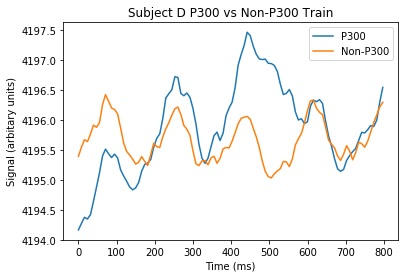
\includegraphics[width=\figureWidth]{images/results/subject_D_p300.jpg}
    \caption{Subject D \ac{p300} plot.}
    \label{fig:subject-D-p300}
\end{figure}
\clearpage
% ----------------------------------------------------------------

Table \ref{tab:subject-C-D-char-reco} shows the character recognition analysis for subjects C and D using the 14 channels of EMOTIV EPOCH+ Headset (Figure \ref{fig:emotiv-14-channels}).\par
\begin{table}[!ht]
    \centering
    \begin{tabular}{ c | c | c | c | c | c || c}
        \hline
        \textbf{Classifier} & \textbf{Channels} & \textbf{Window} & \textbf{Filters} & \textbf{A} & \textbf{B} & \textbf{Average} \\
        \hline\hline
        \multirow{4}{*}{\textbf{LDA}} & 14 & $0 \to 800ms$ & - & $53.36$ & $53.36$ & $53.36$\%\\
        {} & 14 & $0 \to 800ms$ & CarMaZsD & $86.67$ & $60$ & $73.33\pm13.33$\%\\
        {} & 14 & $200 \to 600ms$ & - & $46.67$ & $46.67$ & $46.67$\%\\
        {} & 14 & $200 \to 600ms$ & CarMaZsD & $46.67$ & $46.67$ & $46.67$\%\\
        \hline
    \end{tabular}
    \caption{Subject C and D character recognition rate.}
    \label{tab:subject-C-D-char-reco}
\end{table}
% ----------------------------------------------------------------
\clearpage
% ================================================================
\chapter{Conclusion and Future Work}
\label{chap:conclusion}
% ================================================================
\section{Conclusion}
In conclusion, using \ac{p300} based \ac{bci} a \ac{p300} speller was programmed. Using \ac{ml} and specifically \ac{lda} classifier, a character recognition rate of around 80\% in the competition's dataset and 70\% in the recorded dataset was achieved. The number of channels didn't have much effect, at least it depends on the subject, their brain waves and their state of mind \ref{tab:subject-A-B-char-reco}.\par
% ----------------------------------------------------------------
However, one could see that applying filters did have great impact on the character recognition rate. As shown in Table \ref{tab:subject-C-D-char-reco}, an increase of around 20\% was achieved on subject C, however, on subject D there was no effect at all, mainly due to signal interference, lack of attention and lack of experience with the platform. One can see that effect from the \ac{p300} plot in Figure \ref{fig:subject-C-p300} versus Figure \ref{fig:subject-D-p300}.\par
% ----------------------------------------------------------------

\section{Future Work}
There is a lot can be done to increase the efficiency of this project. Such as trying different combinations of filters and classifiers for each subject since \ac{ml} models are like maths problems where one can achieve the desired answer with more than one way.\par
% ----------------------------------------------------------------
An auto-complete functionality can be added as well in order to save time. one character takes around 30 seconds to be determined. If we consider the average of one word to be 5 characters, then, this will take around 150 seconds in total which is a lot for one word. However, if auto-complete was added it can take half the time to determine what the user wants thus saving a lot of time.\par
% ----------------------------------------------------------------
Sentence's prediction and adaptability can be added as well. As it can check what the user tends to type so often then add it as a shortcut instead of typing the whole sentence from the beginning and predicting next word within the current sentence (same behavior as mobile keyboards).\par
% ----------------------------------------------------------------
A mobile phone application can be programmed as well since \ac{p300} speller does not require much computation. However, it will be hard to do it on mobile phones with small screens or older version platforms since it might not be compatible with the headset.

\clearpage
% ================================================================
\appendix
\renewcommand{\appendixtocname}{Appendix}
\renewcommand{\appendixpagename}{\appendixtocname}
\addappheadtotoc
\setboolean{@twoside}{false}
\appendixpage

\chapter{Lists}
\addcontentsline{toc}{section}{List of Abbreviations}
\begin{acronym}[\hspace{3cm}]
    \acro{bci}[BCI]{Brain–Computer Interface \cite{inbook1}}
    \acro{bmi}[BMI]{Brain-Machine Interface}
    \acro{car}[CAR]{Common Average Reference \cite{inproceedings1, inproceedings2, article2}}
    \acro{dbi}[DBI]{Direct Brain Interface}
    \acro{decimation}{Decimation \cite{inproceedings1, inproceedings2, article1, article2}}
    \acro{ecog}[ECoG]{Electrocorticogram \cite{inbook1}}
    \acro{eeg}[EEG]{Electroencephalography \cite{inbook1}}
    \acro{erp}[ERP]{Event Related Potential}
    \acro{gui}[GUI]{Graphical User Interface}
    \acro{icr}[ICR]{Intracortical Recordings \cite{inbook1}}
    \acro{lda}[LDA]{Linear Discriminant Analysis}
    \acro{ma}{Moving Average \cite{inproceedings1, inproceedings2, article1}}
    \acro{ml}[ML]{Machine Learning \cite{article7}}
    \acro{p300}[P300]{Peak 300 \cite{article3}}
    \acro{sci}[SCI]{Spinal Cord Injury}
    \acro{ssvep}[SSVEP]{Steady State Visually Evoked Potential
    \cite{article4}}
    \acro{zscore}{Z-Score \cite{inproceedings1, article2}}
\end{acronym}
\clearpage


\listoffigures
\addcontentsline{toc}{section}{List of Figures}
\clearpage


\listoftables
\addcontentsline{toc}{section}{List of Tables}
\clearpage


%\listofalgorithms
%\addcontentsline{toc}{section}{List of Algorithms}
%\clearpage

\renewcommand\bibname{References}
\bibliographystyle{ieeetr}
\bibliography{bibtex/references.bib}
\addcontentsline{toc}{chapter}{References}

\end{document}